% AutoKaggle wide (explore) and narrow (exploit) search loops.
% Build: pdflatex search-loops.tex && pdftocairo -svg search-loops.pdf search-loops.svg
\documentclass[tikz,border=8pt]{standalone}
\usepackage[scaled]{helvet}
\renewcommand\familydefault{\sfdefault}
\usepackage[T1]{fontenc}
\usepackage{amssymb}
\usetikzlibrary{positioning,fit,backgrounds,arrows.meta,calc,shapes.geometric,decorations.pathreplacing}

\definecolor{ink}{HTML}{1F2937}
\definecolor{muted}{HTML}{6B7280}
\definecolor{wideC}{HTML}{2563EB}
\definecolor{narrowC}{HTML}{0F766E}
\definecolor{svcC}{HTML}{475569}
\definecolor{okC}{HTML}{15803D}
\definecolor{noC}{HTML}{B91C1C}
\definecolor{loopC}{HTML}{D97706}

\tikzset{
  every node/.style={font=\footnotesize, text=ink},
  panel/.style={draw=#1!55, fill=#1!5, rounded corners=4pt, line width=0.6pt},
  ptitle/.style={font=\small\bfseries, text=#1!80!black, anchor=north west},
  box/.style={draw=#1!70, fill=white, rounded corners=3pt, line width=0.6pt,
              align=center, inner sep=4pt, minimum height=0.95cm},
  dec/.style={draw=#1!70, fill=white, diamond, aspect=2.1, line width=0.6pt,
              align=center, inner sep=1pt, font=\scriptsize},
  flow/.style={-{Stealth[length=2.2mm]}, line width=0.6pt, draw=muted},
  lbl/.style={font=\scriptsize\itshape, text=muted, fill=white, inner sep=1.5pt},
  yes/.style={font=\scriptsize\bfseries, text=okC!80!black, fill=white, inner sep=1.5pt},
  no/.style={font=\scriptsize\bfseries, text=noC!80!black, fill=white, inner sep=1.5pt},
  chip/.style={draw=svcC!70, fill=white, rounded corners=2.5pt, minimum width=1.5cm,
               minimum height=0.6cm, font=\scriptsize\bfseries},
}
\newcommand{\sub}[1]{\\[-1pt]{\scriptsize\color{muted}#1}}

\begin{document}
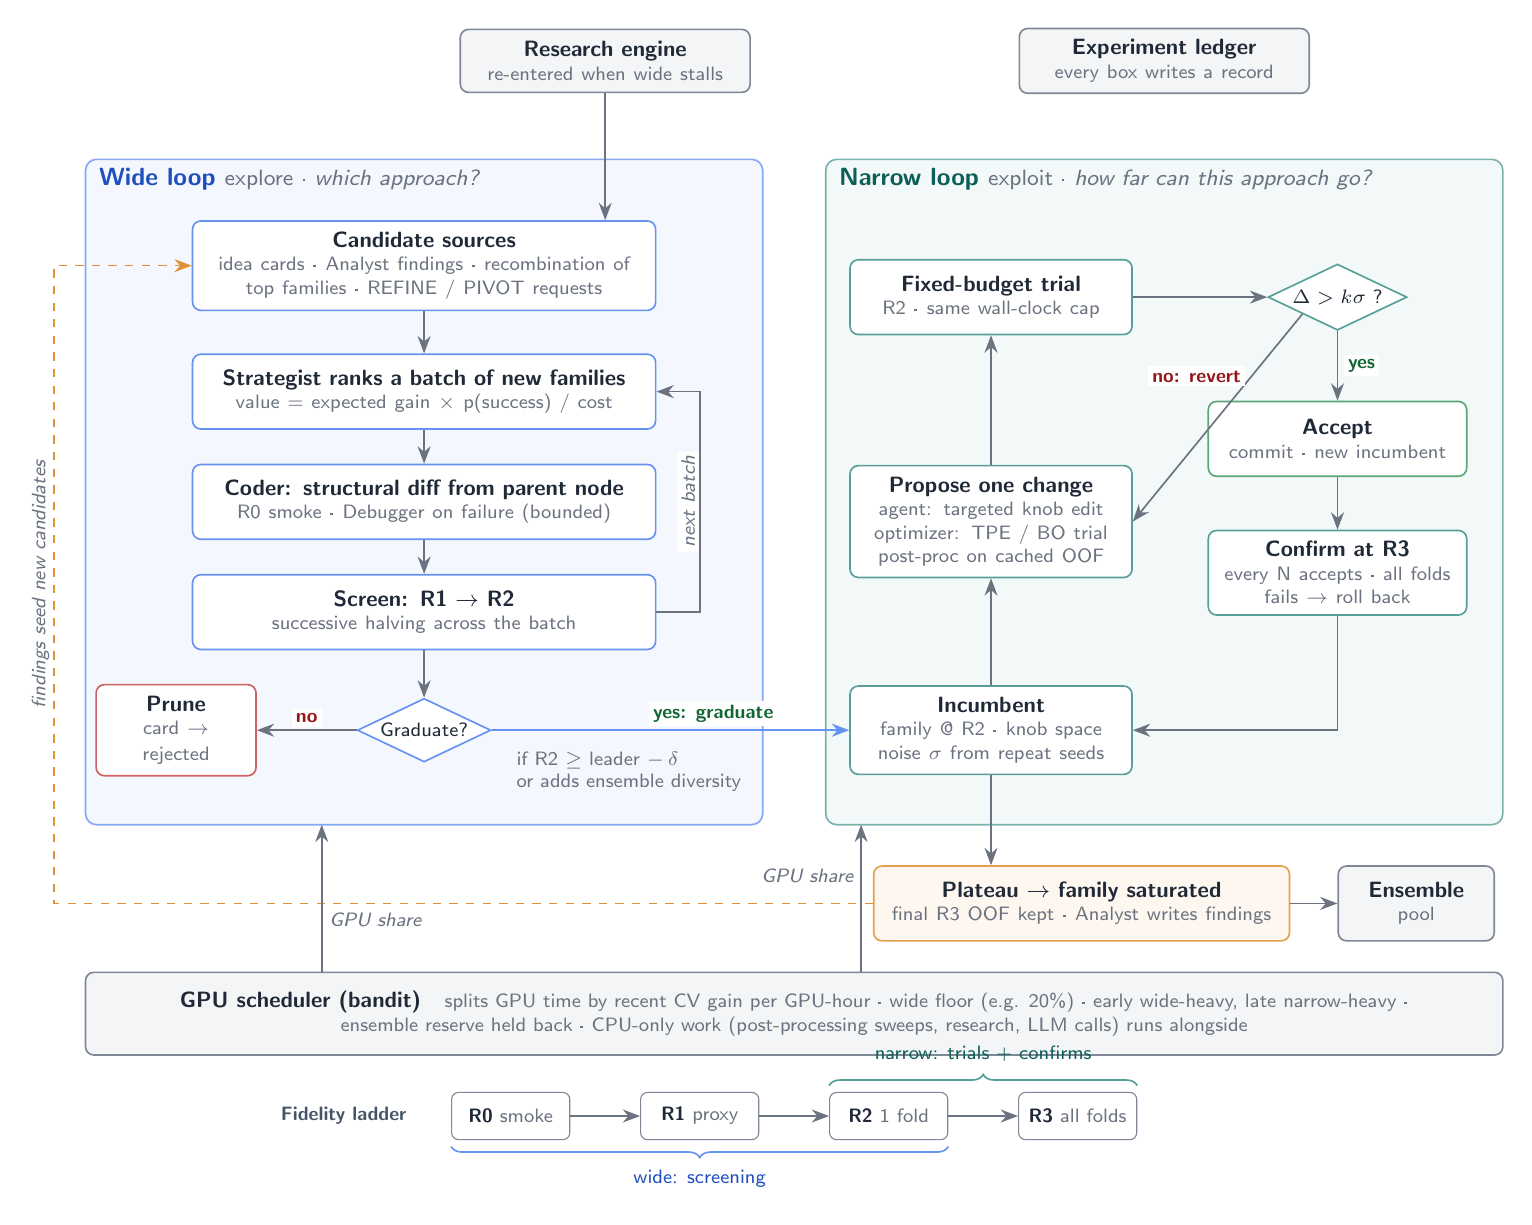
\begin{tikzpicture}

% ======================= WIDE LOOP =======================
\node[box=wideC, text width=5.6cm] (ws) at (4.3,-1.35)
  {\textbf{Candidate sources}\sub{idea cards · Analyst findings · recombination of}\sub{top families · REFINE / PIVOT requests}};
\node[box=wideC, text width=5.6cm] (wr) at (4.3,-2.95)
  {\textbf{Strategist ranks a batch of new families}\sub{value = expected gain $\times$ p(success) / cost}};
\node[box=wideC, text width=5.6cm] (wc) at (4.3,-4.35)
  {\textbf{Coder: structural diff from parent node}\sub{R0 smoke · Debugger on failure (bounded)}};
\node[box=wideC, text width=5.6cm] (wsc) at (4.3,-5.75)
  {\textbf{Screen: R1 $\rightarrow$ R2}\sub{successive halving across the batch}};
\node[dec=wideC] (wg) at (4.3,-7.25) {Graduate?};
\node[box=noC, text width=1.75cm, minimum height=0.8cm] (prune) at (1.15,-7.25)
  {\textbf{Prune}\sub{card $\rightarrow$ rejected}};

\draw[flow] (ws) -- (wr);
\draw[flow] (wr) -- (wc);
\draw[flow] (wc) -- (wsc);
\draw[flow] (wsc) -- (wg);
\draw[flow] (wg.west) -- node[no, above=1pt] {no} (prune.east);
\draw[flow] (wsc.east) -- ++(0.55,0) |- node[lbl, pos=0.25, rotate=90, anchor=south] {next batch} (wr.east);

\begin{scope}[on background layer]
  \node[panel=wideC, fit={(0,0) (8.6,-8.45)}, inner sep=0pt] (widepanel) {};
\end{scope}
\node[ptitle=wideC] at (widepanel.north west) {\,Wide loop \textnormal{\textcolor{muted}{\footnotesize explore · \emph{which approach?}}}};

% graduation rule note
\node[font=\scriptsize, text=muted, align=left, anchor=north west] at (5.35,-7.4)
  {if R2 $\geq$ leader $-\,\delta$\\or adds ensemble diversity};

% ======================= NARROW LOOP =======================
\node[box=narrowC, text width=3.3cm] (ni) at (11.5,-7.25)
  {\textbf{Incumbent}\sub{family @ R2 · knob space}\sub{noise $\sigma$ from repeat seeds}};
\node[box=narrowC, text width=3.3cm] (np) at (11.5,-4.6)
  {\textbf{Propose one change}\sub{agent: targeted knob edit}\sub{optimizer: TPE / BO trial}\sub{post-proc on cached OOF}};
\node[box=narrowC, text width=3.3cm] (nr) at (11.5,-1.75)
  {\textbf{Fixed-budget trial}\sub{R2 · same wall-clock cap}};
\node[dec=narrowC] (nd) at (15.9,-1.75) {$\Delta > k\sigma$ ?};
\node[box=okC, text width=3.0cm] (na) at (15.9,-3.55)
  {\textbf{Accept}\sub{commit · new incumbent}};
\node[box=narrowC, text width=3.0cm] (nc) at (15.9,-5.25)
  {\textbf{Confirm at R3}\sub{every N accepts · all folds}\sub{fails $\rightarrow$ roll back}};

\draw[flow] (ni) -- (np);
\draw[flow] (np) -- (nr);
\draw[flow] (nr) -- (nd);
\draw[flow] (nd) -- node[yes, right=2pt] {yes} (na);
\draw[flow] (na) -- (nc);
\draw[flow] (nc.south) |- (ni.east);
\draw[flow] (nd.south west) -- node[no, pos=0.3, left=2pt] {no: revert} (np.east);

\begin{scope}[on background layer]
  \node[panel=narrowC, fit={(9.4,0) (18,-8.45)}, inner sep=0pt] (narrowpanel) {};
\end{scope}
\node[ptitle=narrowC] at (narrowpanel.north west) {\,Narrow loop \textnormal{\textcolor{muted}{\footnotesize exploit · \emph{how far can this approach go?}}}};

% graduation crosses between loops
\draw[flow, line width=0.9pt, draw=wideC!70] (wg.east) ++(0,0) -- node[yes, above=1pt, pos=0.62] {yes: graduate} (ni.west);

% ======================= ABOVE: research =======================
\node[box=svcC, fill=svcC!6, text width=3.4cm, minimum height=0.8cm] (research) at (6.6,1.25)
  {\textbf{Research engine}\sub{re-entered when wide stalls}};
\draw[flow] (research.south) -- (research.south |- ws.north);

\node[box=svcC, fill=svcC!6, text width=3.4cm, minimum height=0.8cm] (ledger) at (13.7,1.25)
  {\textbf{Experiment ledger}\sub{every box writes a record}};

% ======================= BELOW: exit, scheduler, ladder =======================
\node[box=loopC, fill=loopC!6, text width=5.0cm] (sat) at (12.65,-9.45)
  {\textbf{Plateau $\rightarrow$ family saturated}\sub{final R3 OOF kept · Analyst writes findings}};
\node[box=svcC, fill=svcC!6, text width=1.7cm] (ens) at (16.9,-9.45) {\textbf{Ensemble}\sub{pool}};
\draw[flow] (ni.south) -- (ni.south |- sat.north);
\draw[flow] (sat.east) -- (ens.west);
\draw[flow, dashed, draw=loopC!80] (sat.west) -- (-0.4,-9.45) |- node[lbl, pos=0.25, rotate=90, anchor=south] {findings seed new candidates} (ws.west);

\node[draw=svcC!70, fill=svcC!6, rounded corners=3pt, line width=0.6pt, minimum width=18cm,
      minimum height=1.05cm, align=center] (sched) at (9,-10.85)
  {\textbf{GPU scheduler (bandit)}\quad\textcolor{muted}{\scriptsize splits GPU time by recent CV gain per GPU-hour · wide floor (e.g. 20\%) · early wide-heavy, late narrow-heavy ·}\\[-1pt]
   \textcolor{muted}{\scriptsize ensemble reserve held back · CPU-only work (post-processing sweeps, research, LLM calls) runs alongside}};
\draw[flow] (sched.north -| 3.0,0) -- node[lbl, right=1pt, pos=0.35] {GPU share} (3.0,-8.45);
\draw[flow] (sched.north -| 9.85,0) -- node[lbl, left=1pt, pos=0.65] {GPU share} (9.85,-8.45);

% ladder
\def\yL{-12.15}
\node[font=\scriptsize\bfseries, text=svcC, anchor=east] at (4.2,\yL) {Fidelity ladder};
\foreach \r/\d [count=\i from 0] in {R0/smoke,R1/proxy,R2/1 fold,R3/all folds}{
  \node[chip] (r\i) at (5.4+\i*2.4,\yL) {\r\ {\normalfont\color{muted}\d}};
}
\foreach \i [evaluate=\i as \j using int(\i+1)] in {0,1,2}{ \draw[flow] (r\i) -- (r\j); }
\draw[decorate, decoration={brace, mirror, amplitude=4pt}, draw=wideC!70, line width=0.6pt]
  ($(r0.south west)+(0,-0.08)$) -- ($(r2.south east)+(0,-0.08)$)
  node[midway, below=5pt, font=\scriptsize, text=wideC!80!black] {wide: screening};
\draw[decorate, decoration={brace, amplitude=4pt}, draw=narrowC!70, line width=0.6pt]
  ($(r2.north west)+(0,0.08)$) -- ($(r3.north east)+(0,0.08)$)
  node[midway, above=5pt, font=\scriptsize, text=narrowC!80!black] {narrow: trials + confirms};

\end{tikzpicture}
\end{document}
